\newcolumntype{+}{>{\global\let\currentrowstyle\relax}}
\newcolumntype{^}{>{\currentrowstyle}}
\newcommand{\rowstyle}[1]{\gdef\currentrowstyle{#1}%
#1\ignorespaces
}

\chapter{Experiments and Results}
\label{sec:impl}

\section{Window Size Selection}
\label{sec:windowSize}

The size of the window (i.e. 9x9 pixels) affects the quality of the disparity map (see Figure~\ref{fig:tsukubaWinSize}) and the number of computations required to create the disparity map. The 3x3 window size in Figure~\ref{fig:tsukuba3x3} will be processed the fastest  out of the window sizes shown since each SAD calculation only has 9 pairs of pixels compared to say the 13x13 window, or 169 pairs of pixels in Figure~\ref{fig:tsukuba13x13}. The 13x13 window has the least amount of noise, in its disparity map, but it also loses some detail as shown by the lamp in the foreground of the image compared to the other images. Also, as the window size gets larger, more resources are needed on the FPGA board. The 7x7 and 9x9 window sizes were used because they both were reasonably compromising on the amount of noise in the disparity maps and the amount of hardware resources needed for implementation. 

\begin{figure}
\begin{center}
	\begin{subfigure}{0.45\textwidth}
		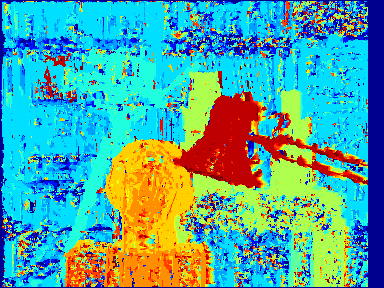
\includegraphics[width=\textwidth]{figures/sad_tsukuba_3x3_0-15.png}
		\caption{SAD 3x3 Window Disparity Map}
		\label{fig:tsukuba3x3}
	\end{subfigure}
	\begin{subfigure}{0.45\textwidth}
		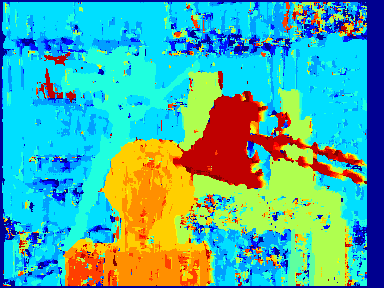
\includegraphics[width=\textwidth]{figures/sad_tsukuba_5x5_0-15.png}
		\caption{SAD 5x5 Window Disparity Map}
		\label{fig:tsukuba5x5}
	\end{subfigure}
	\\
	\begin{subfigure}{0.45\textwidth}
		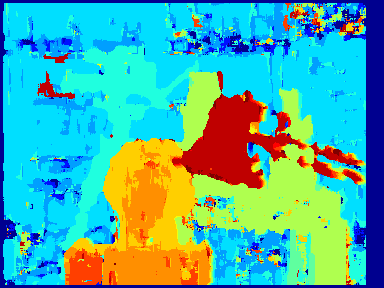
\includegraphics[width=\textwidth]{figures/sad_tsukuba_7x7_0-15.png}
		\caption{SAD 7x7 Window Disparity Map}
		\label{fig:tsukuba7x7}
	\end{subfigure}
	\begin{subfigure}{0.45\textwidth}
		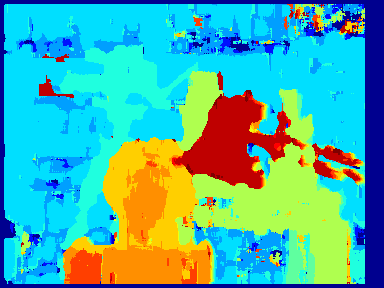
\includegraphics[width=\textwidth]{figures/sad_tsukuba_9x9_0-15.png}
		\caption{SAD 9x9 Window Disparity Map}
		\label{fig:tsukuba9x9}
	\end{subfigure}
	\\
	\begin{subfigure}{0.45\textwidth}
		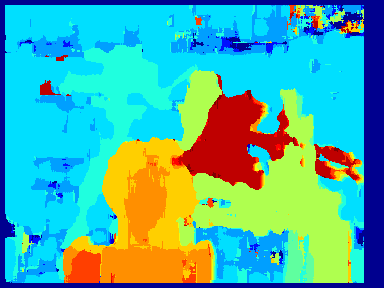
\includegraphics[width=\textwidth]{figures/sad_tsukuba_11x11_0-15.png}
		\caption{SAD 11x11 Window Disparity Map}
		\label{fig:tsukuba11x11}
	\end{subfigure}
	\begin{subfigure}{0.45\textwidth}
		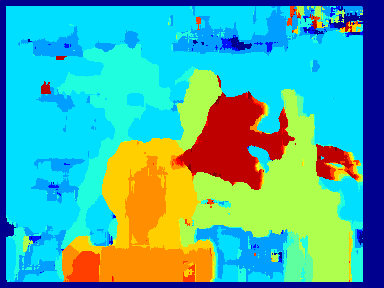
\includegraphics[width=\textwidth]{figures/sad_tsukuba_13x13_0-15.png}
		\caption{SAD 13x13 Window Disparity Map}
		\label{fig:tsukuba13x13}
	\end{subfigure}
	\captionfonts
	\caption{Window size comparisons for disparity maps~\cite{matlab} of the Tskukuba image pair~\cite{middlebury}.}
	\label{fig:tsukubaWinSize}
\end{center}
\end{figure}


\section{Resource Utilization on FPGA}
\label{sec:utilize}

See Table~\ref{table:utilize} in Appendix~\ref{sec:appdxE}. The 7x7 window implementation actually uses more resources on the FPGA board than the 9x9 window implementation due to the amount of parallel calculations used in the SAD algorithm. There is still plenty of space on the board for other types of top level designs that could use this SAD module.


\section{Testbench Simulation}
\label{sec:testbench}

See Figure~\ref{fig:tb_9x9} and Figure~\ref{fig:tb_7x7} in Appendix~\ref{sec:appdxF} for the testbench simulations for the 9x9 window and 7x7 window implementations, respectively.

The h2fvalid\_i value near the top of the figure is high when image data is being written to the SAD wrapper. The first section that is high is the initial rows being sent to the wrapper. The smaller following sections that are high are the next row being sent to the wrapper. The wrapper has been designed to allow both the template image data and the search image data to be sent to the wrapper at the same time, thus reducing the amount of time taken to get all necessary data into the wrapper. When the signal f2hready\_i goes high, it means that the disparity values are being sent out of the wrapper. 

\subsection{9x9 Window Implementation Runtime}
\label{sec:testbench9x9}

Based on the testbench simulation in Fig.~\ref{fig:tb_9x9} the theoretical frames per second can be inferred for different image sizes. The simulation assumes the 100MHz clock on the FPGA is used, and thus each clock cycle is 10 ns long.

According to the testbench simulation, for a 9x9 window with 4 pixels being processed in parallel, the first section includes the initial image data given to the SAD wrapper up to the when the the corresponding disparity values come out, takes 3.35 us. After that, a constant cycle is produced that has the SAD wrapper take in the next row and produces the next disparity values, which takes 1.22 us. A 640x480 image has 307,200 pixels, which will produce a disparity map of 617x472, which is 291,224 pixels. Disparity values are not produced for pixels that either the windows cannot fit on or there is not enough room for the 16 SAD values to be calculated for pixel. Since 4 pixels are processed in parallel, 291,224 pixels is divided by 4 pixels/iteration, giving 72,806 iterations. So, 72,806 iterations times 1.22 us/iteration plus 3.35 us (initial section, hence minus one on number of iterations) gives 88,826.67 us or approximately 0.0888 seconds per frame. Therefore, an image size of 640x480 can be processed at around 11.26 frames per second. Table~\ref{table:tb_9x9} shows the theoretical frame rate for the image sizes used in this chapter.

\begin{table}
	\begin{center}
		\begin{tabular}{|c|c|c|c|}
			\hline 
				\rowstyle{\bfseries} Image Width & 
				\rowstyle{\bfseries} Image Height & 
				\rowstyle{\bfseries} Seconds/frame & 
				\rowstyle{\bfseries} Frames/second
			\tabularnewline
			\hline 
			640 & 480 & 0.0888 & 11.26
			\tabularnewline
			\hline 
			384 & 288 & 0.0308 & 32.43
			\tabularnewline
			\hline 
			434 & 383 & 0.0470 & 21.27
			\tabularnewline
			\hline 			
			\end{tabular}
		\captionfonts
		\caption{9x9 window for theoretical runtime for the FPGA board for different image sizes.}
		\label{table:tb_9x9}
	\end{center}
\end{table}

\subsection{7x7 Window Implementation Runtime}
\label{sec:testbench7x7}

Based on the testbench simulation in Fig.~\ref{fig:tb_7x7} the theoretical frames per second (fps) can be inferred for different image sizes. The simulation assumes the 100MHz clock on the FPGA is used, and thus each clock cycle is 10 ns long.

According to the testbench simulation, for a 7x7 window with 2 pixels being processed in parallel, the first section includes the initial image data given to the SAD wrapper up to the when the the corresponding disparity values come out, takes 1.78 us. After that, a constant cycle is produced that has the SAD wrapper take in the next row and produces the next disparity values, which takes 0.42 us. A 640x480 image has 307,200 pixels, which will produce a disparity map of 619x474, which is 293,406 pixels. Disparity values are not produced for pixels that either the windows cannot fit on or there is not enough room for the 16 SAD values to be calculated for pixel. Since 2 pixels are processed in parallel, 293,406 pixels is divided by 2 pixels/iteration, giving 146,703 iterations. So, 146,703 iterations times 0.42 us/iteration plus 1.78 us (initial section, hence minus one on number of iterations) gives 61,617.04 us or approximately 0.0616 seconds per frame. Therefore, an image size of 640x480 can be processed at around 16.23 frames per second. Table~\ref{table:tb_7x7} shows the theoretical frame rate for the image sizes used in this chapter.


\begin{table}
	\begin{center}
		\begin{tabular}{|c|c|c|c|}
			\hline 
				\rowstyle{\bfseries} Image Width & 
				\rowstyle{\bfseries} Image Height & 
				\rowstyle{\bfseries} Seconds/frame & 
				\rowstyle{\bfseries} Frames/second
			\\ \hline 
			640 & 480 & 0.0616 & 16.23
			\\ \hline 
			384 & 288 & 0.0215 & 46.51
			\\ \hline 
			434 & 383 & 0.0327 & 30.58
			\\ \hline 
		\end{tabular}	
		\captionfonts
		\caption{7x7 window for theoretical runtime for the FPGA board for different image sizes.}
		\label{table:tb_7x7}
	\end{center}
\end{table}

\section{Test Image Pairs}
\label{sec:runtime}

In this section, FPGA disparity maps are compared to disparity maps created using Python. The SAD algorithm implementation in Python is show in Appendix~\ref{sec:appdxD}. The Python SAD version is performed completely in serial, so 1 pixel at a time. It is run on a desktop that (COMPUTER SPECS) running Ubuntu 64-bit.

\subsection{Data Overflows}
\label{sec:overflow}

In VHDL, the code for the hardware to be generated is designed. The size of the data used for storing logic and variables is defined during the coding process. In the SAD algorithm, it is possible for the SAD value to become much larger than the individual pixel values. For example, the pixel values range from 0 to 255, or 2\textsuperscript{8} bits, while some SAD value could be over 4,095, or need more than 2\textsuperscript{12}. Most SAD values were under 4,096, however, to account for those that were above it, the SAD algorithm use 2\textsuperscript{14} bits to account for any values from 0 to 16,383. Figure~\ref{fig:overflow} shows what can happen when the data size allotted for the SAD algorithm is not large enough (i.e. only having 2\textsuperscript{10} bits of space). The data used is unsigned, so when it goes above the highest supported value, it goes back to 0 and continues from there. 

Since most of the values were below 4,096, a measure was put in place in order to reduce the amount of bits needed during the minimum comparisons. If a SAD value was greater than 4,095, then 4,095 was returned for the calculated SAD because the greater the value, the less likely that search pixel is the correct corresponding one to the template pixel. In Figure~\ref{fig:tsukubaDispMap} and Figure~\ref{fig:venusDispMap}, the only real noticeable difference in the Python to FPGA comparisons is at the top of the images. The colors, warmer is closer and cooler is farther away, show that the top areas are thought to be closer than they actually are in the FPGA images. For a robot, it would be better to err on the side of thinking an object is closer than it actually is because the robot will be less prone to collide with the object. If a robot thought an object was farther away than it actually was, then the likelihood of collision would increase.

\begin{figure}
	\begin{center}
		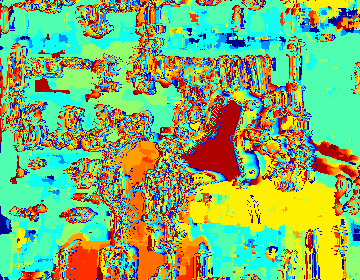
\includegraphics[width=80mm]{figures/tsukuba_disp9x9_2_sad_overflow.png}
		\captionfonts
		\caption{Data overflow for Tskukuba image pair ~\cite{middlebury}.}
		\label{fig:overflow}
	\end{center}
\end{figure}

\subsection{Tsukuba}
\label{sec:tsukuba}

In Figure~\ref{fig:tsukubaL} and Figure~\ref{fig:tsukubaR}, the Tsukuba image pair are shown. Figure~\ref{fig:tsukubaDispMap} shows how the 7x7 window implementation is slightly noisier than the 9x9 window implementation. As discussed in Section~\ref{sec:overflow}, the only noticeable difference between the Python implementation and the FPGA implementation is at the top of the disparity maps. This is caused by the two images not having similar enough corresponding regions, which causes SAD values to be greater than normal.

\begin{figure}
\begin{center}
	\begin{subfigure}{0.45\textwidth}
		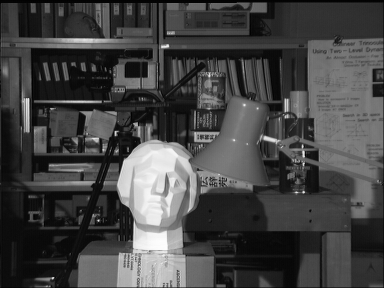
\includegraphics[width=\textwidth]{figures/tsukubaL.jpg}
		\caption{Left Tsukuba Grayscale Image}
		\label{fig:tsukubaL}
	\end{subfigure}
	\begin{subfigure}{0.45\textwidth}
		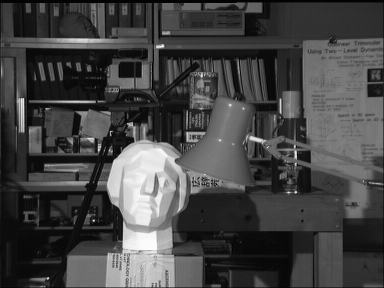
\includegraphics[width=\textwidth]{figures/tsukubaR.jpg}
		\caption{Right Tsukuba Grayscale Image}
		\label{fig:tsukubaR}
	\end{subfigure}
	\\
	\begin{subfigure}{0.45\textwidth}
		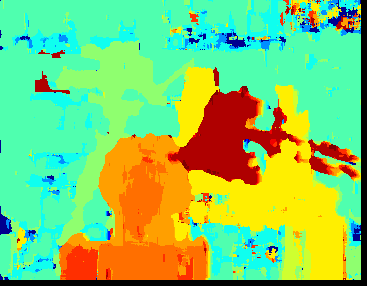
\includegraphics[width=\textwidth]{figures/tsukuba_9x9_python3.png}
		\caption{Python3 9x9 Disparity Map}
		\label{fig:tsukubaPy}
	\end{subfigure}
	\begin{subfigure}{0.45\textwidth}
		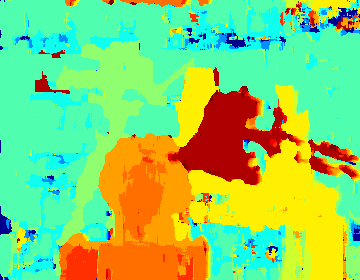
\includegraphics[width=\textwidth]{figures/tsukuba_9x9_fpga.png}
		\caption{FPGA 9x9 Disparity Map}
		\label{fig:tsukubaFPGA}
	\end{subfigure}
	\\
	\begin{subfigure}{0.45\textwidth}
		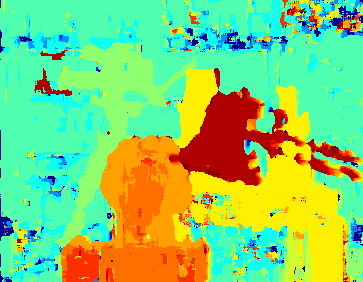
\includegraphics[width=\textwidth]{figures/tsukuba_7x7_python3.png}
		\caption{Python3 7x7 Disparity Map}
		\label{fig:tsukubaPy}
	\end{subfigure}
	\begin{subfigure}{0.45\textwidth}
		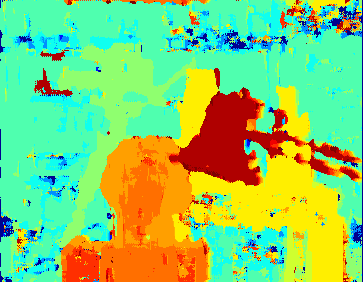
\includegraphics[width=\textwidth]{figures/tsukuba_7x7_fpga.png}
		\caption{FPGA 7x7 Disparity Map}
		\label{fig:tsukubaFPGA}
	\end{subfigure}
	\captionfonts
	\caption{Disparity map comparison of the Tskukuba image pair ~\cite{middlebury}.}
	\label{fig:tsukubaDispMap}
\end{center}
\end{figure}

\subsection{Venus}
\label{sec:venus}

In Figure~\ref{fig:venusL} and Figure~\ref{fig:venusR}, the Venus image pair are shown. In the image pair, the newspaper articles are flat and slanted, relative to the cameras. This gradual slope, also present in the background, can be difficult for the SAD algorithm to deal with, however, the algorithm is still able to give a fairly accurate representation of the depth in the image. It also causes the gradient pattern shown in the disparity maps. The 7x7 window depth maps have more noise than the 9x9 window depth maps.

\begin{figure}
\begin{center}
	\begin{subfigure}{0.45\textwidth}
		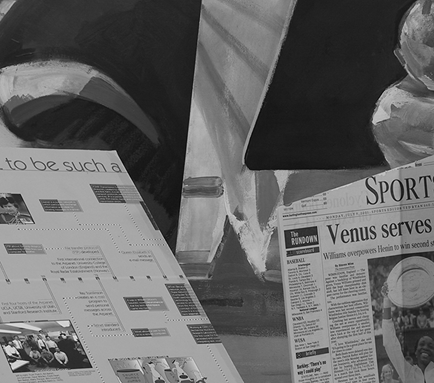
\includegraphics[width=\textwidth]{figures/venusL.png}
		\caption{Left Venus Grayscale Image}
		\label{fig:venusL}
	\end{subfigure}
	\begin{subfigure}{0.45\textwidth}
		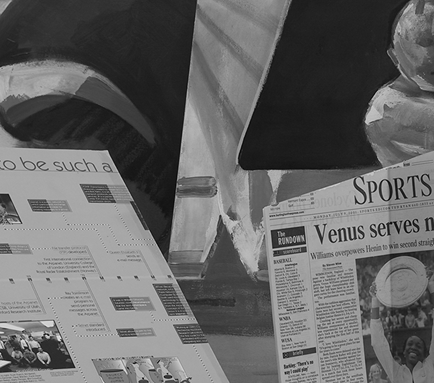
\includegraphics[width=\textwidth]{figures/venusR.png}
		\caption{Right Venus Grayscale Image}
		\label{fig:venusR}
	\end{subfigure}
	\\
	\begin{subfigure}{0.45\textwidth}
		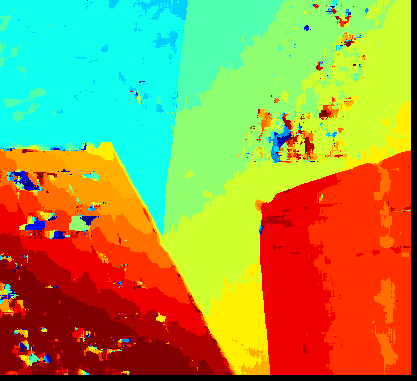
\includegraphics[width=\textwidth]{figures/venus_9x9_python3.png}
		\caption{Python3 9x9 Disparity Map}
		\label{fig:venusPy}
	\end{subfigure}
	\begin{subfigure}{0.45\textwidth}
		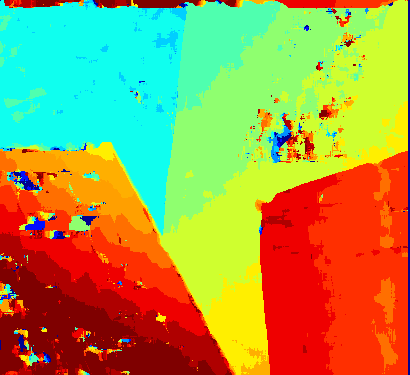
\includegraphics[width=\textwidth]{figures/venus_9x9_fpga.png}
		\caption{FPGA 9x9 Disparity Map}
		\label{fig:venusFPGA}
	\end{subfigure}
	\\
	\begin{subfigure}{0.45\textwidth}
		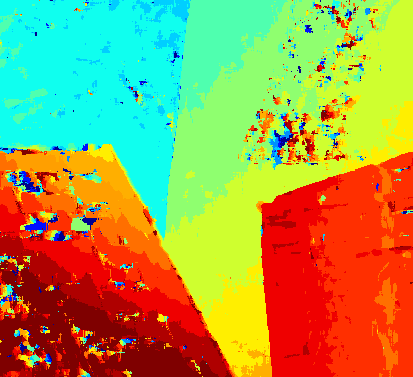
\includegraphics[width=\textwidth]{figures/venus_7x7_python3.png}
		\caption{Python3 7x7 Disparity Map}
		\label{fig:venusPy}
	\end{subfigure}
	\begin{subfigure}{0.45\textwidth}
		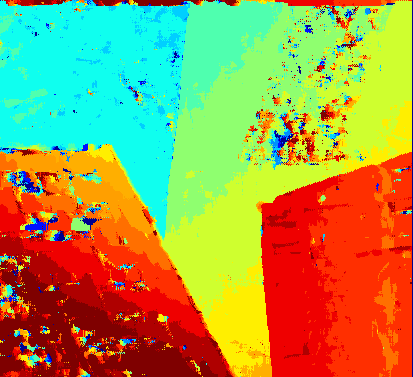
\includegraphics[width=\textwidth]{figures/venus_7x7_fpga.png}
		\caption{FPGA 7x7 Disparity Map}
		\label{fig:venusFPGA}
	\end{subfigure}
	\captionfonts
	\caption{Disparity map comparison of the Venus image pair ~\cite{middlebury}.}
	\label{fig:venusDispMap}
\end{center}
\end{figure}


\subsection{Cones}
\label{sec:cones}

In Figure~\ref{fig:conesL} and Figure~\ref{fig:conesR}, the Venus image pair are shown. Figure~\ref{fig:conesDispMap} shows the issue of objects in an image pair being too close to the stereo cameras. The closer an objects is to the stereo cameras, the greater its disparity value will be. Using the SAD algorithm with a 9x9 window and a disparity range of 60 (as opposed to the range of 16 used on the FPGA board) produces the results in Figure~\ref{fig:conesMatlab}. When the disparity range is not high enough, the disparity map in Figure~\ref{fig:conesPy} is produced.

\begin{figure}
\begin{center}
	\begin{subfigure}{0.45\textwidth}
		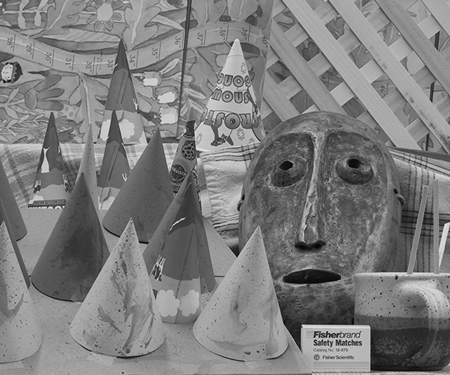
\includegraphics[width=\textwidth]{figures/conesL.png}
		\caption{Left Cones Grayscale Image}
		\label{fig:conesL}
	\end{subfigure}
	\begin{subfigure}{0.45\textwidth}
		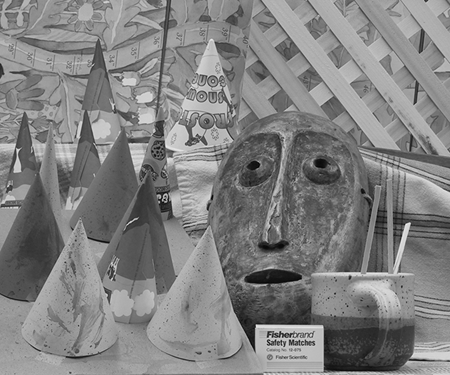
\includegraphics[width=\textwidth]{figures/conesR.png}
		\caption{Right Cones Grayscale Image}
		\label{fig:conesR}
	\end{subfigure}
	\\
	\begin{subfigure}{0.45\textwidth}
		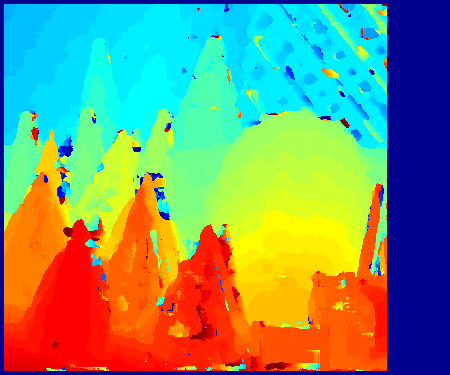
\includegraphics[width=\textwidth]{figures/cones_9x9_matlab_0-59.png}
		\caption{9x9 at Disparity Range of 60 ~\cite{matlab}}
		\label{fig:conesMatlab}
	\end{subfigure}
	\begin{subfigure}{0.45\textwidth}
		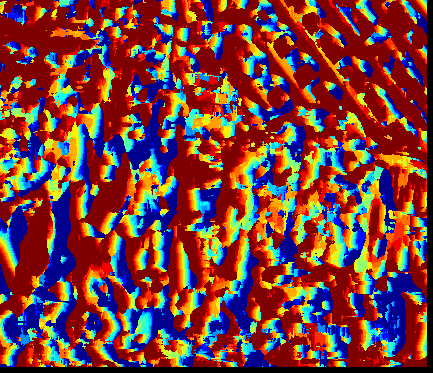
\includegraphics[width=\textwidth]{figures/cones_9x9_python3.png}
		\caption{9x9 at Disparity Range of 16}
		\label{fig:conesPy}
	\end{subfigure}
	\captionfonts
	\caption{Disparity map comparison of the Cones image pair ~\cite{middlebury}.}
	\label{fig:conesDispMap}
\end{center}
\end{figure}




